\documentclass{ximera}
\graphicspath{  %% When looking for images,
{./}            %% look here first,
{./pictures/}   %% then look for a pictures folder,
{../pictures/}  %% which may be a directory up.
{../../pictures/}  %% which may be a directory up.
{../../../pictures/}  %% which may be a directory up.
{../../../../pictures/}  %% which may be a directory up.
}

\usepackage{listings}
%\usepackage{circuitikz}
\usepackage{xcolor}
\usepackage{amsmath,amsthm}
\usepackage{subcaption}
\usepackage{graphicx}
\usepackage{tikz}
%\usepackage{tikz-3dplot}
\usepackage{amsfonts}
%\usepackage{mdframed} % For framing content
%\usepackage{tikz-cd}

  \renewcommand{\vector}[1]{\left\langle #1\right\rangle}
  \newcommand{\arrowvec}[1]{{\overset{\rightharpoonup}{#1}}}
  \newcommand{\ro}{\texttt{R}}%% row operation
  \newcommand{\dotp}{\bullet}%% dot product
  \renewcommand{\l}{\ell}
  \let\defaultAnswerFormat\answerFormatBoxed
  \usetikzlibrary{calc,bending}
  \tikzset{>=stealth}
  




%make a maroon color
\definecolor{maroon}{RGB}{128,0,0}
%make a dark blue color
\definecolor{darkblue}{RGB}{0,0,139}
%define the color fourier0 to be the maroon color
\definecolor{fourier0}{RGB}{128,0,0}
%define the color fourier1 to be the dark blue color
\definecolor{fourier1}{RGB}{0,0,139}
%define the color fourier 1t to be the light blue color
\definecolor{fourier1t}{RGB}{173,216,230}
%define the color fourier2 to be the dark green color
\definecolor{fourier2}{RGB}{0,100,0}
%define teh color fourier2t to be the light green color
\definecolor{fourier2t}{RGB}{144,238,144}
%define the color fourier3 to be the dark purple color
\definecolor{fourier3}{RGB}{128,0,128}
%define the color fourier3t to be the light purple color
\definecolor{fourier3t}{RGB}{221,160,221}
%define the color fourier0t to be the red color
\definecolor{fourier0t}{RGB}{255,0,0}
%define the color fourier4 to be the orange color
\definecolor{fourier4}{RGB}{255,165,0}
%define the color fourier4t to be the darker orange color
\definecolor{fourier4t}{RGB}{255,215,0}
%define the color fourier5 to be the yellow color
\definecolor{fourier5}{RGB}{255,255,0}
%define the color fourier5t to be the darker yellow color
\definecolor{fourier5t}{RGB}{255,255,100}
%define the color fourier6 to be the green color
\definecolor{fourier6}{RGB}{0,128,0}
%define the color fourier6t to be the darker green color
\definecolor{fourier6t}{RGB}{0,255,0}

%New commands for this doc for errors in copying
\newcommand{\eigenvar}{\lambda}
%\newcommand{\vect}[1]{\mathbf{#1}}
\renewcommand{\th}{^{\text{th}}}
\newcommand{\st}{^{\text{st}}}
\newcommand{\nd}{^{\text{nd}}}
\newcommand{\rd}{^{\text{rd}}}
\newcommand{\paren}[1]{\left(#1\right)}
\newcommand{\abs}[1]{\left|#1\right|}
\newcommand{\R}{\mathbb{R}}
\newcommand{\C}{\mathbb{C}}
\newcommand{\Hilb}{\mathbb{H}}
\newcommand{\qq}[1]{\text{#1}}
\newcommand{\Z}{\mathbb{Z}}
\newcommand{\N}{\mathbb{N}}
\newcommand{\q}[1]{\text{``#1''}}
%\newcommand{\mat}[1]{\begin{bmatrix}#1\end{bmatrix}}
\newcommand{\rref}{\text{reduced row echelon form}}
\newcommand{\ef}{\text{echelon form}}
\newcommand{\ohm}{\Omega}
\newcommand{\volt}{\text{V}}
\newcommand{\amp}{\text{A}}
\newcommand{\Seq}{\textbf{Seq}}
\newcommand{\Poly}{\textbf{P}}
\renewcommand{\quad}{\text{    }}
\newcommand{\roweq}{\simeq}
\newcommand{\rowop}{\simeq}
\newcommand{\rowswap}{\leftrightarrow}
\newcommand{\Mat}{\textbf{M}}
\newcommand{\Func}{\textbf{Func}}
\newcommand{\Hw}{\textbf{Hamming weight}}
\newcommand{\Hd}{\textbf{Hamming distance}}
\newcommand{\rank}{\text{rank}}
\newcommand{\longvect}[1]{\overrightarrow{#1}}
% Define the circled command
\newcommand{\circled}[1]{%
  \tikz[baseline=(char.base)]{
    \node[shape=circle,draw,inner sep=2pt,red,fill=red!20,text=black] (char) {#1};}%
}

% Define custom command \strikeh that just puts red text on the 2nd argument
\newcommand{\strikeh}[2]{\textcolor{red}{#2}}

% Define custom command \strikev that just puts red text on the 2nd argument
\newcommand{\strikev}[2]{\textcolor{red}{#2}}

%more new commands for this doc for errors in copying
\newcommand{\SI}{\text{SI}}
\newcommand{\kg}{\text{kg}}
\newcommand{\m}{\text{m}}
\newcommand{\s}{\text{s}}
\newcommand{\norm}[1]{\left\|#1\right\|}
\newcommand{\col}{\text{col}}
\newcommand{\sspan}{\text{span}}
\newcommand{\proj}{\text{proj}}
\newcommand{\set}[1]{\left\{#1\right\}}
\newcommand{\degC}{^\circ\text{C}}
\newcommand{\centroid}[1]{\overline{#1}}
\newcommand{\dotprod}{\boldsymbol{\cdot}}
%\newcommand{\coord}[1]{\begin{bmatrix}#1\end{bmatrix}}
\newcommand{\iprod}[1]{\langle #1 \rangle}
\newcommand{\adjoint}{^{*}}
\newcommand{\conjugate}[1]{\overline{#1}}
\newcommand{\eigenvarA}{\lambda}
\newcommand{\eigenvarB}{\mu}
\newcommand{\orth}{\perp}
\newcommand{\bigbracket}[1]{\left[#1\right]}
\newcommand{\textiff}{\text{ if and only if }}
\newcommand{\adj}{\text{adj}}
\newcommand{\ijth}{\emph{ij}^\text{th}}
\newcommand{\minor}[2]{M_{#2}}
\newcommand{\cofactor}{\text{C}}
\newcommand{\shift}{\textbf{shift}}
\newcommand{\startmat}[1]{
  \left[\begin{array}{#1}
}
\newcommand{\stopmat}{\end{array}\right]}
%a command to give a name to explorations and hints and theorems
\newcommand{\name}[1]{\begin{centering}\textbf{#1}\end{centering}}
\newcommand{\vect}[1]{\vec{#1}}
\newcommand{\dfn}[1]{\textbf{#1}}
\newcommand{\transpose}{\mathsf{T}}
\newcommand{\mtlb}[2][black]{\texttt{\textcolor{#1}{#2}}}
\newcommand{\RR}{\mathbb{R}} % Real numbers
\newcommand{\id}{\text{id}}
\newcommand{\coord}[1]{\langle#1\rangle}
\newcommand{\RREF}{\text{RREF}}
\newcommand{\Null}{\text{Null}}
\newcommand{\Nullity}{\text{Nullity}}
\newcommand{\Rank}{\text{Rank}}
\newcommand{\Col}{\text{Col}}
\newcommand{\Ef}{\text{EF}}
\newcommand{\boxprod}[3]{\abs{(#1\times#2)\cdot#3}}

\author{Zack Reed} %PEter Selinger
\title{Bringing Everything Together: Gauss and Echelon Forms}
\begin{document}
\begin{abstract}
Here we introduce one of the most prevalent applications of matrices and vectors, the solving of systems of equations.
\end{abstract}
\maketitle
    
\section*{Systems, Augmented Matrices and Elementary Row Operations}
 
\subsection*{Augmented Matrices}
 
We've been focusing on a few solution-preserving operations that can be carried out on systems of equations, called \emph{row operations}:
\begin{itemize}
\item Switching the order of equations $i$ and $j$: $R_i\leftrightarrow R_j$
\item Multiplying both sides of an equation by the same non-zero constant $\lambda$, $R_i\rightarrow\lambda R_i$
\item Adding a multiple of one equation to another, $R_i\rightarrow R_i+\lambda R_j$
\end{itemize}
 
 
In SECTIONBLAH we tied these row operations to special, reversible matrices called \emph{elementary matrices}:

\begin{itemize}

  \item The \textbf{row swapping matrix} $E_{ij}$, the identity matrix with rows $i$ and $j$ swapped.
  
  $E_{12}$ performed on a $3\times 3$ matrix would be the matrix

  \begin{equation*}
    \begin{bmatrix}
      0 & 1 & 0 \\
      1 & 0 & 0 \\
      0 & 0 & 1
    \end{bmatrix}
  \end{equation*}

  \item The \textbf{scaling matrix} $E_{i}(c)$ is the matrix that results from multiplying row $i$ of the identity matrix by the scalar $c$.
  
  $E_{2}(3)$ performed on a $3\times 3$ matrix would be the matrix

  \begin{equation*}
    \begin{bmatrix}
      1 & 0 & 0 \\
      0 & 3 & 0 \\
      0 & 0 & 1
    \end{bmatrix}.
  \end{equation*}

  \item The \textbf{row addition matrix} $E_{ij}(c)$ is the matrix that results from adding $c$ times row $i$ to row $j$ of the identity matrix.
  
  $E_{3,2}(2)$ performed on a $3\times 3$ matrix would be the matrix

  \begin{equation*}
    \begin{bmatrix}
      1 & 0 & 0 \\
      0 & 1 & 0 \\
      0 & 2 & 1
    \end{bmatrix}.
  \end{equation*}

  This will add $2$ times the second row to the third row.

\end{itemize}
 
In this section, we explicitly draw connections between these two representations of the same operations, and seek an efficient method for simplifying a system so that a solution (if it exists) is determinable.
 
\begin{exploration}
Consider the linear system
\begin{equation}
  \begin{array}{ccccccccc}
      x &- &y&&&&&= &0 \\
     2x& -&2y&+&z&+&2w&=&4\\
     & &y&&&+&w&=&0\\
     & &&&2z&+&w&=&5
  \end{array}
\end{equation}

Our goal is to use elementary row operations to transform this system into an equivalent and solvable system of the form

\begin{equation}\begin{array}{ccccccccc}
      x & &&&&&&= &a \\
     & &y&&&&&=&b\\
     & &&&z&&&=&c\\
     & &&&&&w&=&d
    \end{array}
    \end{equation}  
  
We'll first perform these steps as we have been, using row operations, and then perform the same operations with elementary matrices, on what's called an \emph{augmented matrix} representation of the system.

We start by subtracting twice row 1 from row 2. ($R_2\rightarrow R_2-2R_1$)
 
$$\begin{matrix}
      x &- &y&+&0z&+&0w&= &0 \\
     0x& +&0y&+& 1z&+& 2w&=& 4\\
     0x& +&y&+&0z&+&w&=&0\\
     0x&+&0y&+&2z&+&w&=&5
    \end{matrix}$$

Next, we add row 3 to row 1. ($R_1\rightarrow R_1+R_3$) 

\begin{prompt}
 $$\begin{matrix}
      x &+ & \answer{0}y&+&\answer{0}z&+& \answer{1}w&= & \answer{0} \\
     0x& +&0y&+&z&+&2w&=&4\\
     0x& +&y&+&0z&+&w&=&0\\
     0x&+&0y&+&2z&+&w&=&5
    \end{matrix}$$
\end{prompt}


\begin{prompt} Subtract twice row 2 from row 4. ($R_4\rightarrow R_4-2R_2$)
$$\begin{matrix}
      x &+ &0y&+&0z&+&1w&= &0 \\
     0x& +&0y&+&z&+&2w&=&4\\
     0x& +&y&+&0z&+&w&=&0\\
     \answer{0}x&+&\answer{0}y&+& \answer{0}z&+& \answer{-3}w&=& \answer{-3}
    \end{matrix}$$
\end{prompt}

\begin{prompt} Divide row 4 by $-3$. ($R_4\rightarrow -\frac{1}{3}R_4$)
$$\begin{matrix}
      x &+ &0y&+&0z&+&1w&= &0 \\
     0x& +&0y&+&z&+&2w&=&4\\
     0x& +&y&+&0z&+&w&=&0\\
     \answer{0}x&+&\answer{0}y&+&\answer{0}z&+& \answer{1}w&=&\answer{1}
    \end{matrix}$$
\end{prompt}   

\begin{prompt} We will do three operations in one step.
$$R_1\rightarrow R_1-R_4$$
$$R_2\rightarrow R_2-2R_4$$
$$R_3\rightarrow R_3-R_4$$
$$\begin{matrix}
      x &+ &\answer{0}y&+&\answer{0}z&+& \answer{0}w&= & \answer{-1} \\
     \answer{0}x& +&\answer{0}y&+&\answer{1}z&+& \answer{0}w&=& \answer{2}\\
     \answer{0}x& +&\answer{1}y&+&\answer{0}z&+& \answer{0}w&=& \answer{-1}\\
     0x&+&0y&+&0z&+&1w&=&1
    \end{matrix}$$
\end{prompt}   

We now exchange rows 2 and 3. ($R_2\leftrightarrow R_3$)
\begin{equation}\label{eq:sys20rref1}
\begin{array}{ccccccccc}
      x &+ &0y&+&0z&+&0w&= &-1 \\
   0x& +&y&+&0z&+&0w&=&-1\\
   0x& +&0y&+&z&+&0w&=&2\\
     0x&+&0y&+&0z&+&w&=&1
    \end{array}
    \end{equation}
    If we drop all of the zero terms, we have:
    \begin{equation}\label{eq:sys20rrefnozeros}
    \begin{array}{ccccccccc}
      x & &&&&&&= &-1 \\
   & &y&&&&&=&-1\\
   & &&&z&&&=&2\\
     &&&&&&w&=&1
    \end{array}
    \end{equation}
Now we see that $(-1, -1, 2, 1)$ is the solution.
 
If we were to state this as matrix equations, this would be the matrix-vector Multiplications

$$M\vec{x}=\vec{b}$$

where $M_1$ is the matrix 

\begin{equation}
  M_1=\begin{bmatrix}
    1 & -1 & 0 & 0 \\
    2 & -2 & 1 & 2 \\
    0 & 1  & 0 & 1 \\
    0 & 0  & 2 & 1 \\
  \end{bmatrix}
\end{equation},

$\vec{x}$ is the vector

\begin{equation}
  \vec{x}=\begin{bmatrix}
    -1 \\
    -1  \\
    2 \\
    1  
  \end{bmatrix}
\end{equation},

and $\vec{b}$ is the vector

\begin{equation}
  \vec{b}=\begin{bmatrix}
    0 \\
    4  \\
    0 \\
    5  
  \end{bmatrix}
\end{equation}.

That's a key interpretation of the variables $x, y, z, w$ satisfying the system, is that the matrix-vector multiplication gives the vector represented by the right side of the equations.

\begin{remark}{MATLAB Check!}

  Let's check it in MATLAB! We can set up the matrix 

  \begin{verbatim}
    
    M=[1, -1, 0, 0;
        2, -2, 1, 2;
        0, 0, 2, 1]

  \end{verbatim}

  Then, we set up the potential solution vector 

  \begin{verbatim}
  
    x=[-1; -1; 2; 1]

  \end{verbatim}

  Then, we multiply $M*x$ and hope that it's $\vec{b}$!

  \begin{verbatim}
  
    b=M*x

  \end{verbatim}

  Thankfully, we get the right solution vector!

\end{remark}

This matrix-interpretation of the solution will become much more important in the next chapter, but for now we're going to use it to give us some slight notational convenience. 

\begin{remark}{Augmented Matrices}



\end{remark}


$$\left[\begin{array}{cccc|c} 
 1&-1&0&0&0\\2&-2&1&2&4\\0&1&0&1&0\\0&0&2&1&5
 \end{array}\right]$$
  
   The side to the left of the vertical bar is called the \dfn{coefficient matrix}, while the side to the right of the bar is a vector that consists of constants on the right side of the system.  The coefficient matrix, together with the vector, is called an \dfn{augmented matrix}.
  
 We can capture all of the elementary row operations we performed earlier as follows:
 
$$\left[\begin{array}{cccc|c} 
 1&-1&0&0&0\\2&-2&1&2&4\\0&1&0&1&0\\0&0&2&1&5
 \end{array}\right]
 \begin{array}{c}
 \\
 \xrightarrow{R_2-2R_1}\\
\\
\\
 \end{array}
 \left[\begin{array}{cccc|c} 
 1&-1&0&0&0\\0&0&1&2&4\\0&1&0&1&0\\0&0&2&1&5
 \end{array}\right]
 \begin{array}{c}
 \xrightarrow{R_1+R_3}\\
 \\
\\
\\
 \end{array}$$
 $$\left[\begin{array}{cccc|c} 
 1&0&0&1&0\\2&-2&1&2&4\\0&1&0&1&0\\0&0&2&1&5
 \end{array}\right]
 \begin{array}{c}
 \\
 \\
\\
\xrightarrow{R_4-2R_2}\\
 \end{array}
 \left[\begin{array}{cccc|c} 
 1&0&0&1&0\\0&0&1&2&4\\0&1&0&1&0\\0&0&0&-3&-3
 \end{array}\right]
 \begin{array}{c}
 \\
 \\
\\
\xrightarrow{(-1/3)R_4}\\
 \end{array}$$
 $$\left[\begin{array}{cccc|c} 
 1&0&0&1&0\\0&0&1&2&4\\0&1&0&1&0\\0&0&0&1&1
 \end{array}\right]
 \begin{array}{c}
 \xrightarrow{R_1-R_4}\\
 \xrightarrow{R_2-2R_4}\\
\xrightarrow{R_3-R_4}\\
\\
 \end{array}\left[\begin{array}{cccc|c} 
 1&0&0&0&-1\\0&0&1&0&2\\0&1&0&0&-1\\0&0&0&1&1
 \end{array}\right]\begin{array}{c}
 \\
 \xrightarrow{R_2\leftrightarrow R_3}\\
\\
\\
 \end{array}$$
  
  
  
  
  
  
 \begin{equation}\label{eq:sys20rref}\left[\begin{array}{cccc|c} 
 1&0&0&0&-1\\0&1&0&0&-1\\0&0&1&0&2\\0&0&0&1&1
 \end{array}\right]\end{equation}
  
 The last augmented matrix corresponds to systems in (\ref{eq:sys20rref1}) and (\ref{eq:sys20rrefnozeros}), and we can easily see the solution.  
 
 
\end{exploration}
 
Exploration \ref{init:augmentedmatrixex} introduced us to some vocabulary terms.  Let's formalize our definitions.  Every linear system
$$\begin{array}{ccccccccc}
      a_{11}x_1 &+ &a_{12}x_2&+&\ldots&+&a_{1n}x_n&= &b_1 \\
     a_{21}x_1 &+ &a_{22}x_2&+&\ldots&+&a_{2n}x_n&= &b_2 \\
     &&&&\vdots&&&& \\
     a_{m1}x_1 &+ &a_{m2}x_2&+&\ldots&+&a_{mn}x_n&= &b_m
    \end{array}$$
    can be written in the \dfn{augmented matrix form} as follows:
    $$\left[\begin{array}{cccc|c} 
 a_{11}&a_{12}&\ldots&a_{1n}&b_1\\a_{21}&a_{22}&\ldots&a_{2n}&b_2\\\vdots&\vdots&\ddots&\vdots&\vdots\\a_{m1}&a_{m2}&\ldots&a_{mn}&b_m
 \end{array}\right]$$
 The array to the left of the vertical bar is called the \dfn{coefficient matrix} of the linear system and is often given a capital letter name, like $A$.  The vertical array to the right of the bar is called a \dfn{constant vector}.
 $$A=\begin{bmatrix}a_{11}&a_{12}&\ldots&a_{1n}\\a_{21}&a_{22}&\ldots&a_{2n}\\\vdots&\vdots&\ddots&\vdots\\a_{m1}&a_{m2}&\ldots&a_{mn}\end{bmatrix}\quad\text{and}\quad\vec{b}=\begin{bmatrix}b_1\\b_2\\\vdots\\b_m\end{bmatrix}$$
We will sometimes use the following notation to represent an augmented matrix.
 
$$\left[\begin{array}{c|c} 
 A & \vec{b}\\
 \end{array}\right]$$
The same elementary row operations that we perform on a system of equations can be performed on the corresponding augmented matrix, or any matrix for that matter.  If a matrix can be obtained from another matrix by means of elementary row operations, we say that the two matrices are \dfn{row-equivalent}. 
\begin{exploration}\label{init:backsub}
Consider the system
$$\begin{array}{ccccccc}
      x_1 &- &x_2&-&3x_3&= &1 \\
   4x_1& -&2x_2&-&7x_3&=&1\\
   -x_1& +&x_2&+&4x_3&=&1
    \end{array}$$
Recall that in Exploration \ref{init:augmentedmatrixex} we converted the given system to an augmented matrix form, then performed elementary row operations until we arrived at a ``convenient" form.  We then converted the ``convenient" augmented matrix back to a system of equations and identified the solution.  The term ``convenient" is open to interpretation.  In this problem we will explore two ``convenient" forms.  Each one will lead to a definition. 
 
\begin{align}&\left[\begin{array}{ccc|c} 
 1&-1&-3&1\\4&-2&-7&1\\-1&1&4&1
 \end{array}\right]\nonumber\\
 \begin{array}{c}
\\
  \xrightarrow{R_2-4R_1}\\
\xrightarrow{R_3+R_1}\\
 \end{array}
 &\left[\begin{array}{ccc|c} 
 1&-1&-3&1\\0&2&5&-3\\0&0&1&2
 \end{array}\right]\label{eq:sys20rowechelon}\\
 \begin{array}{c}
 \\
 \xrightarrow{(1/2)R_2}\\
\\
\end{array}
&\left[\begin{array}{ccc|c} 
 1&-1&-3&1\\0&1&5/2&-3/2\\0&0&1&2
 \end{array}\right]\nonumber\\
 \begin{array}{c}
 \xrightarrow{R_1+R_2}\\
 \\
\\
\end{array}&\left[\begin{array}{ccc|c} 
 1&0&-1/2&-1/2\\0&1&5/2&-3/2\\0&0&1&2
 \end{array}\right]\nonumber\\
 \begin{array}{c}
 \xrightarrow{R_1+ (1/2)R_3}\\
 \xrightarrow{R_2- (5/2)R_3}\\
\\
\end{array}
&\left[\begin{array}{ccc|c} 
 1&0&0&1/2\\0&1&0&-13/2\\0&0&1&2
 \end{array}\right]\label{eq:sys20reducedrowechelon}
 \end{align}
 
The augmented matrix in (\ref{eq:sys20reducedrowechelon}) has the same convenient form as the one in (\ref{eq:sys20rref}).  This augmented matrix corresponds to the system
\begin{equation*}
    \begin{array}{ccccccc}
      x_1 & &&&&= &1/2 \\
   & &x_2&&&=&-13/2\\
   & &&&x_3&=&2
        \end{array}
    \end{equation*}
This gives us the solution $(\frac{1}{2}, -\frac{13}{2}, 2)$.
 
While the augmented matrix in (\ref{eq:sys20reducedrowechelon}) was certainly ``convenient", we could have converted back to the equation format a little earlier.  Let's take a look at the augmented matrix in (\ref{eq:sys20rowechelon}).  Converting (\ref{eq:sys20rowechelon}) to a system of equations gives us
\begin{equation*}
    \begin{array}{ccccccc}
      x_1 &- &x_2&-&3x_3&= &1\\
   & &2x_2&+&5x_3&=&-3\\
   & &&&x_3&=&2
        \end{array}
    \end{equation*}
Substituting $x_3=2$ into the second equation and solving for $x_2$ gives us $$x_2=\frac{-3-5(2)}{2}=-\frac{13}{2}$$  Now substituting $x_3=2$ and $x_2=-\frac{13}{2}$ into the first equation results in $$x_1=1+\left(-\frac{13}{2}\right)+3(2)=\frac{1}{2}$$  This process is called \dfn{back substitution} and it produces the same solution as we obtained earlier.
\end{exploration}
 
Observe that the coefficient matrices in (\ref{eq:sys20rref}) and (\ref{eq:sys20reducedrowechelon}) have the same format: 1's along the diagonal, zeros above and below the 1's.  The other ``convenient" format, exhibited by the coefficient matrix in (\ref{eq:sys20rowechelon}),  also has zeros below the diagonal, but not all of the diagonal entries are 1's and some of the entries above the diagonal are not zero.  Each of these formats gives rise to a definition.  These definitions are the topic of the next section.
 
 
\subsection*{Row-Echelon and Reduced Row-Echelon Forms}
 
\begin{definition}\label{def:leadentry} The first non-zero entry in a row of a matrix (when read from left to right) is called the \dfn{leading entry}.  When the leading entry is 1, we refer to it as a \dfn{leading 1}.
\end{definition}
 
\begin{definition}[Row-Echelon Form]\label{def:ref}
A matrix is said to be in \dfn{row-echelon form} if:
\begin{enumerate}
\item All entries below each leading entry are 0.
\item Each leading entry is in a column to the right of the leading entries in the rows above it.
\item All rows of zeros, if there are any, are located below non-zero rows.
\end{enumerate}
\end{definition}
 
The term row-echelon form can be applied to matrices whether or not they are augmented matrices (matrices with the vertical bar). For example, both the coefficient matrix and the augmented matrix in (\ref{eq:sys20rowechelon}) are in row-echelon form.  Note that the leading entries form a staircase pattern. All entries below the leading entries are zero, but the entries above the leading entries are not all zero.
 
Below are two more examples of matrices in row-echelon form.  The leading entries of each matrix are boxed.
$$\begin{bmatrix}
 \fbox{1}&2&-1&-5&0&2\\0&0&\fbox{3}&1&2&0\\0&0&0&0&\fbox{1}&0
 \end{bmatrix}\quad\text{and}\quad\begin{bmatrix}
 \fbox{4}&2\\0&\fbox{1}\\0&0
 \end{bmatrix}$$
  
  
 
The difference between the coefficient matrix in  (\ref{eq:sys20rowechelon}) and the coefficient matrix in (\ref{eq:sys20reducedrowechelon}) is that the leading entries of the  matrix in (\ref{eq:sys20reducedrowechelon}) are all 1's, and the matrix has zeros above each leading 1.  This motivates our next definition.
 
\begin{definition}[Reduced Row-Echelon Form]\label{def:rref}
A matrix that is already in \dfn{row-echelon} form is said to be in \dfn{reduced row-echelon form} if:
\begin{enumerate}
\item Each leading entry is $1$
\item All entries {\it above} and below each leading $1$ are $0$
\end{enumerate}
\end{definition}
The following two matrices are in \dfn{reduced row-echelon form}.  Note that there are $0$'
s below and above each leading $1$.
 
$$\begin{bmatrix} 
 \fbox{1}&0&-1&0&1\\0&\fbox{1}&0&0&2\\0&0&0&\fbox{1}&2
 \end{bmatrix}\quad\text{and}\quad\begin{bmatrix}
 \fbox{1}&0\\0&\fbox{1}\\0&0
 \end{bmatrix}$$
  
 When solving linear systems using the augmented matrix notation, our goal will be to transform the augmented matrix $M=[A|\vec{b}]$ into a row-echelon or reduced row-echelon form.  The reduced row-echelon form of $M$ is denoted by
$\mbox{rref}(M)$.  As we transform the augmented matrix $M$ to its reduced row-echelon form, the coefficient matrix $A$ (the matrix to the left of the bar) also gets transformed to its reduced row-echelon form, $\mbox{rref}(A)$.
 
 
 
\begin{example}\label{ex:freevar1} Solve the system of equations or determine that the system is inconsistent.
$$\begin{array}{ccccccccc}
      x &- &2y&+&z&&&= &2 \\
     -2x& +&y&-&z&+&w&=&0\\
     x& +&4y&&&+&w&=&1
    \end{array}$$
\begin{explanation}
We begin by rewriting the system in the augmented matrix form.
$$\left[\begin{array}{cccc|c} 
 1&-2&1&0&2\\-2&1&-1&1&0\\1&4&0&1&1
 \end{array}\right]$$
 Our goal is to convert this matrix to its reduced row-echelon form by means of elementary row operations.  To do this, we will proceed from left to right and use leading entries to wipe out all entries above and below them.
  
 $$\left[\begin{array}{cccc|c} 
 1&-2&1&0&2\\-2&1&-1&1&0\\1&4&0&1&1
 \end{array}\right]
 \begin{array}{c}
 \\
 \xrightarrow{R_2+2R_1}\\
\xrightarrow{R_3-R_1}\\
 \end{array}\left[\begin{array}{cccc|c} 
 1&-2&1&0&2\\0&-3&1&1&4\\0&6&-1&1&-1
 \end{array}\right]\begin{array}{c}
 \\
 \\
\xrightarrow{R_3+2R_2}\\
 \end{array}$$
  
 $$\left[\begin{array}{cccc|c} 
 1&-2&1&0&2\\0&-3&1&1&4\\0&0&1&3&7
 \end{array}\right]
 \begin{array}{c}
 \\
 \xrightarrow{(-1/3)R_2}\\
\\
 \end{array}\left[\begin{array}{cccc|c} 
 1&-2&1&0&2\\0&1&-1/3&-1/3&-4/3\\0&0&1&3&7
 \end{array}\right]\begin{array}{c}
 \xrightarrow{R_1+2R_2}\\
 \\
\\
 \end{array}$$
  
 $$\left[\begin{array}{cccc|c} 
 1&0&1/3&-2/3&-2/3\\0&1&-1/3&-1/3&-4/3\\0&0&1&3&7
 \end{array}\right]
 \begin{array}{c}
 \xrightarrow{R_1-(1/3)R_3}\\
 \xrightarrow{R_2+(1/3)R_3}\\
\\
 \end{array}\left[\begin{array}{cccc|c} 
 1&0&0&-5/3&-3\\0&1&0&2/3&1\\0&0&1&3&7
 \end{array}\right]$$
  
 Our final matrix may not be quite as nice as the one in (\ref{eq:sys20reducedrowechelon}), but it is in reduced row-echelon form.  Our next step is to convert our augmented matrix back to a system of equations.  We have:
 $$\begin{array}{ccccccccc}
      x & &&&&-&(5/3)w&= &-3 \\
     & &y&&&+&(2/3)w&=&1\\
     & &&&z&+&3w&=&7
    \end{array}$$
 We will rewrite the system as follows:
 $$\begin{array}{ccccccccc}
      x & &&&&&&= &-3+(5/3)w \\
     & &y&&&&&=&1-(2/3)w\\
     & &&&z&&&=&7-3w
    \end{array}$$
 Now we see that we can assign any value to $w$, then compute $x$, $y$ and $z$ to obtain a solution to the system.  For example, let $w=0$, then $x=-3$, $y=1$ and $z=7$, so $(-3, 1, 7, 0)$ is a solution.  If we let $w=3$, then $x=2$, $y=-1$ and $z=-2$, so $(2, -1, -2, 3)$ is also a solution.   To capture all possibilities, we will let $w=t$, where $t$ is an arbitrary \dfn{parameter}.  
  
  We can think of the solution set in two different ways.  First, the solution set is the set of all points of the form$$\left(-3+\frac{5}{3}t, 1-\frac{2}{3}t, 7-3t, t\right)$$
  
 We can also think of the solution set in geometric terms by observing that
 \begin{align*}
 x&=-3+\frac{5}{3}t\\
 y&=1-\frac{2}{3}t\\
 z&=7-3t\\
 w&=t
 \end{align*}
 is a set of parametric equations that describes a line in $\RR^4$.  (See Formula \ref{form:paramlinend})  This means that the three hyperplanes given by the equations in the system intersect in a line, producing infinitely many solutions to the system.
 
\end{explanation}
\end{example}
 
Observe that in Example \ref{ex:freevar1}, variables $x$, $y$ and $z$ correspond to the leading $1's$ in the reduced row-echelon.  We say that $x$, $y$ and $z$ are the \dfn{leading variables}.  Variable $w$ is not a leading variable; we refer to it as a \dfn{free variable} and assign a \dfn{parameter} $t$ to it.
 
\begin{example}\label{ex:nosolutionssys}
Solve the system of equations or determine that the system is inconsistent.
$$\begin{array}{ccccccc}
      2x & -&y&&&= &2 \\
     x& +&y&-&2z&=&0\\
     -3x& &&+&2z&=&-1
    \end{array}$$
     
    \begin{explanation}
    We rewrite the system in augmented matrix form and transform it to reduced row-echelon form.  We leave the details of the elementary row operations to the reader and state the final result.
     
   \begin{equation}\label{eq:sys20nosolutionsys} \left[\begin{array}{ccc|c} 
 2&-1&0&2\\1&1&-2&0\\-3&0&2&-1
 \end{array}\right]\begin{array}{c}
 \\
 \rightsquigarrow\\
 \\
 \end{array}\left[\begin{array}{ccc|c} 
 1&0&-2/3&0\\0&1&-4/3&0\\0&0&0&1
 \end{array}\right]\end{equation}
     
 Converting back to a system of linear equations, we get
  
 \begin{equation}\label{eq:sys20nosolutions}\begin{array}{ccccccc}
      0x &+ &0y&-&(2/3)z&= &0 \\
     0x&+ &0y&-&(4/3)z&=&0\\
     0x&+ &0y&+&0z&=&1
    \end{array}\end{equation}
    The last equation in this system clearly has no solutions.  We conclude that this system (and the original system) is inconsistent.
    \end{explanation}
     
\end{example}
 
\begin{observation}\label{ob:inconsistent} Note that the last row of the reduced row-echelon form in (\ref{eq:sys20nosolutionsys}) looks like this
$$\left[\begin{array}{ccc|c} 
 0&0&0&1
 \end{array}\right]$$
 This row corresponds to the equation
 $$\begin{array}{ccccccc}
     0x&+ &0y&+&0z&=&1
    \end{array}$$
 which clearly has no solutions. 
  
 In general, if the reduced row-echelon form of the augmented matrix contains a row
 $$\left[\begin{array}{ccc|c} 
 0&\ldots&0&1
 \end{array}\right]$$
 we can conclude that the system is inconsistent.
\end{observation}
 
\begin{example}\label{ex:rrefinfmanysolutionssys}
Solve the system of equations or determine that the system is inconsistent.
$$\begin{array}{ccccccc}
      x & -&3y&-&z&= &3 \\
     -3x& +&5y&&&=&-2\\
     x&+ &y&+&2z&=&-4
    \end{array}$$
     
    \begin{explanation}
    We rewrite the system in the augmented matrix form and transform it to reduced row-echelon form.  We leave the details of the elementary row operations to the reader and state the final result.
     
   $$ \left[\begin{array}{ccc|c} 
 1&-3&-1&3\\-3&5&0&-2\\1&1&2&-4
 \end{array}\right]\begin{array}{c}
 \\
 \rightsquigarrow\\
 \\
 \end{array}\left[\begin{array}{ccc|c} 
 1&0&5/4&-9/4\\0&1&3/4&-7/4\\0&0&0&0
 \end{array}\right]$$
 Converting the augmented matrix back to a system of equations we get
 $$\begin{array}{ccccccc}
      x &+ &0y&+&(5/4)z&= &-9/4 \\
     0x& +&y&+&(3/4)z&=&-7/4\\
     0x&+ &0y&+&0z&=&0
    \end{array}$$
     
 Unlike the last equation in (\ref{eq:sys20nosolutions}), the last equation in this system has infinitely many solutions because all values of $x$, $y$ and $z$ satisfy it.  Since the last equation contributes nothing, we will remove it and rewrite the system as
 $$\begin{array}{ccccc}
      x & &&= &-9/4-(5/4)z \\
     & &y&=&-7/4-(3/4)z\\
    \end{array}$$
Variables $x$ and $y$ correspond to leading $1's$ in the reduced row-echelon form.  So, $x$ and $y$ are the leading variables.    Variable $z$ is a free variable.  We let $z=t$.  Solutions to this system are points of the form
  $$\left(-\frac{9}{4}-\frac{5}{4}t, -\frac{7}{4}-\frac{3}{4}t, t\right)$$
  We can also interpret the solutions as lying on a line in $\RR^3$ given by parametric equations
  \begin{align*}
  x&=-\frac{9}{4}-\frac{5}{4}t\\
  y&=-\frac{7}{4}-\frac{3}{4}t\\
  z&=t\\
  \end{align*}
   
  This line is the line of intersection of the three planes.
 \end{explanation}
 \end{example}
 
\section*{Practice Problems}
\begin{problem}
Determine whether each augmented matrix shown below is in reduced row-echelon form.
  \begin{problem}\label{prob:rrefmultchoice1}
  $$\left[\begin{array}{cccc|c} 
 0&1&1&0&2\\1&-3&0&1&4\\0&0&1&0&-1
 \end{array}\right]$$
 \begin{multipleChoice}
 \choice{Yes}
 \choice[correct]{No}
 \end{multipleChoice}
  \end{problem}
   
   \begin{problem}\label{prob:rrefmultchoice2}
  $$\left[\begin{array}{cc|c} 
 1&1&1\\0&1&0\\0&0&0
 \end{array}\right]$$
 \begin{multipleChoice}
 \choice{Yes}
 \choice[correct]{No}
 \end{multipleChoice}
  \end{problem}
   
  \begin{problem}\label{prob:rrefmultchoice3}
  $$\left[\begin{array}{cc|c} 
 1&0&1\\0&1&0\\0&0&0
 \end{array}\right]$$
 \begin{multipleChoice}
 \choice[correct]{Yes}
 \choice{No}
 \end{multipleChoice}
  \end{problem}
   
  \begin{problem}\label{prob:rrefmultchoice4}
  $$\left[\begin{array}{ccc|c} 
 1&0&1&0\\0&1&0&0\\0&0&0&1
 \end{array}\right]$$
 \begin{multipleChoice}
 \choice[correct]{Yes}
 \choice{No}
 \end{multipleChoice}
  \end{problem}
   
   \begin{problem}\label{prob:rrefmultchoice5}
  $$\left[\begin{array}{ccc|c} 
 1&1&0&2\\0&1&0&9\\0&0&1&-1
 \end{array}\right]$$
 \begin{multipleChoice}
 \choice{Yes}
 \choice[correct]{No}
 \end{multipleChoice}
  \end{problem}
   
\end{problem}
 
\begin{problem}\label{prob:rrefnosolutionssys}
Fill in the steps that lead to the reduced row-echelon form in Example \ref{ex:nosolutionssys}.
\end{problem}
 
\begin{problem}\label{prob:rreffinfmanysolutionsys}
Fill in the steps that lead to the reduced row-echelon form in Example \ref{ex:rrefinfmanysolutionssys}.
\end{problem}
 
\begin{problem} \label{prob:numberofsolutionsmultch}
Suppose a system of equations has the following reduced row-echelon form
  $$\left[\begin{array}{ccc|c} 
 1&0&0&4\\0&1&-3&-6\\0&0&0&1
 \end{array}\right]$$
 What can you say about the system?
 \begin{multipleChoice}
 \choice[correct]{The system is inconsistent}
 \choice{The system has infinitely many solutions}
 \choice{The system has a unique solution}
 \choice{We would have to examine the original system to make the final determination}
 \end{multipleChoice}
  \end{problem}
\begin{problem}
Solve each system of equations
\begin{problem}\label{prob:sys20solvesys1}
$$\begin{array}{ccccccc}
      x & +&3y&-&2z&= &-11 \\
     2x& +&y&+&4z&=&12\\
     x& -&y&-&z&=&0
    \end{array}$$
     
    Solution:
    $$( \answer{1}, \answer{-2}, \answer{3})$$
\end{problem}
 
\begin{problem}\label{prob:sys20solvesys2}
$$\begin{array}{ccccccc}
      3x & -&y&+&z&= &-5 \\
     x& +&2y&-&z&=&-3\\
     x& -&5y&+&3z&=&1
    \end{array}$$
     
    Solution: (Enter your answers in fraction form)
    $$\left(\answer{-13/7}-\answer{1/7}t, \answer{-4/7}+\answer{4/7}t, t\right)$$
\end{problem}
\end{problem}
 
\section*{Example Source}
 
Linear system in Exploration \ref{init:augmentedmatrixex} comes from Jim Hefferon's \href{http://joshua.smcvt.edu/linearalgebra/#current_version}{\it Linear Algebra}. (CC-BY-NC-SA)
 
Jim Hefferon, {\it Linear Algebra}, 3rd edition, page 6.

\section*{Gaussian Elimination and Rank}
\subsection*{Row Echelon and Reduced Row Echelon Forms}
 
In \href{https://ximera.osu.edu/oerlinalg/LinearAlgebra/SYS-0020/main}{Augmented Matrix Notation and Elementary Row Operations}, we learned to write linear systems in \dfn{augmented matrix} form and use elementary row operations to transform an augmented matrix to \dfn{row-echelon form} and the \dfn{reduced row-echelon form} in order to solve linear systems. 
 
Recall that a matrix (or augmented matrix) is in \dfn{row-echelon form} if:
\begin{itemize}
\item All entries {\it below} each leading entry are $0$.
\item Each leading entry is in a column to the right of the leading entries in the rows above it.
\item All rows of zeros, if there are any, are located below non-zero rows.
\end{itemize}
 
A matrix in row-echelon form is said to be in \dfn{reduced row-echelon form} if it has the following additional properties
\begin{itemize}
\item Each leading entry is a $1$
\item All entries {\it above} each leading $1$ are $0$
\end{itemize}
 
 
Matrices in row-echelon form and reduced row-echelon form are ``convenient" because their corresponding systems of equations are easy to solve. 
 
In this module we turn to the question of existence and uniqueness of the two echelon forms.  Can every matrix (augmented matrix) be carried to a row-echelon form?  If so, is the row-echelon form unique?  Can every matrix be reduced to a reduced row-echelon form?  If so, is the reduced row-echelon form unique?  The answers we find will have long-lasting implications.
 
 
\begin{exploration}\label{init:gaussianelim1}
Solve the following system of equations.
$$\begin{array}{ccccccccc}
      x &+ &2y&-&3z&= &1 \\
     -5x& +&2y&-&3z&=&1\\
      x&- &2y&+&z&=&1
    \end{array}$$
 
We create an augmented matrix corresponding to the system and apply row operations until the matrix is in row-echelon form. 
$$\left[\begin{array}{ccc|c} 
 1&2&-3&1\\-5&2&-3&1\\1&-2&1&1
 \end{array}\right]
 \begin{array}{c}
 \\
 \xrightarrow{R_2+5R_1}\\
 \xrightarrow{R_3-R_1}\\
 \end{array}
\left[\begin{array}{ccc|c} 
 1&2&-3&1\\0&12&-18&6\\0&-4&4&0
 \end{array}\right]
 \begin{array}{c}
 \\
 \\
 \xrightarrow{R_3+\frac{1}{3}R_2}\\
 \end{array}$$
 \begin{equation}\label{eq:ref1}
 \left[\begin{array}{ccc|c} 
 1&2&-3&1\\0&12&-18&6\\0&0&-2&2
 \end{array}\right]
\end{equation}
 
Note that the elementary row operations that lead to (\ref{eq:ref1}) were not prescribed.  We may employ row-operations in a different manner and obtain a different matrix in row-echelon form.  For example, suppose for some reason we had begun by switching the first and third rows.
 
$$\left[\begin{array}{ccc|c} 
 1&2&-3&1\\-5&2&-3&1\\1&-2&1&1
 \end{array}\right]
 \begin{array}{c}
 \\
 \xrightarrow{R_1\leftrightarrow R_3}\\
\\
 \end{array}
\left[\begin{array}{ccc|c} 
 1&-2&1&1\\-5&2&-3&1\\1&2&-3&1
 \end{array}\right]
 \begin{array}{c}
 \\
\\
\\
 \end{array}$$
 
Next we would reduce this matrix to row-echelon form, perhaps in this way:
 
$$\left[\begin{array}{ccc|c} 
 1&-2&1&1\\-5&2&-3&1\\1&2&-3&1
 \end{array}\right]
 \begin{array}{c}
 \\
 \xrightarrow{R_2+5R_1}\\
 \xrightarrow{R_3-R_1}\\
 \end{array}
\left[\begin{array}{ccc|c} 
 1&-2&1&1\\0&-8&2&6\\0&4&-4&0
 \end{array}\right]
 \begin{array}{c}
 \\
 \\
 \xrightarrow{R_3+\frac{1}{2}R_2}\\
 \end{array}
$$
\begin{equation}\label{eq:ref2}
 \left[\begin{array}{ccc|c} 
 1&-2&1&1\\0&-8&2&6\\0&0&-3&3
 \end{array}\right]
\end{equation}
 
The augmented matrices in (\ref{eq:ref1}) and (\ref{eq:ref2}) are clearly not the same, but both are in row-echelon form.
 
If we write the systems of equations corresponding to (\ref{eq:ref1}) and (\ref{eq:ref2}), we can employ back substitution to solve them.  The matrix in (\ref{eq:ref1}) corresponds to
$$\begin{array}{ccccccccc}
      x &+ &2y&-&3z&= &1 \\
     & &12y&-&18z&=&6\\
      &&&&-2z&=&2
    \end{array}$$
     
The matrix in (\ref{eq:ref2}) corresponds to   
$$\begin{array}{ccccccccc}
      x &- &2y&+&z&= &1 \\
     & &-8y&+&2z&=&6\\
      &&&&-3z&=&3
    \end{array}$$
     
Because both systems are equivalent to the original system, it is not surprising that back substitution yields the same solution for both systems.
 
$$x=\answer{0},\quad y=\answer{-1},\quad z=\answer{-1}$$
 
%From the last equation we get $z=-1$. 
%Next, from the second equation we have $12y-18(-1)=6$, which yields $y=-1$.
%Finally, the first equation gives us $x+2(-1)-3(-1)=1$.  Solving for $x$ we get $x=0$. 
%Therefore, the solution to the system is $$x=0, y=-1, z=-1$$
%We arrive at a different matrix in row-echelon form, but back-substitution yields the same solution to the system (you should check this):  $$x=0, y=-1, z=-1$$
\end{exploration}
 
It is clear from Exploration \ref{init:gaussianelim1} that a row-echelon form corresponding to a matrix is not unique.  But what about the reduced row-echelon form?
 
\begin{exploration}\label{init:gaussianelim2} In this problem we revisit the system
$$\begin{array}{ccccccccc}
      x &+ &2y&-&3z&= &1 \\
     -5x& +&2y&-&3z&=&1\\
      x&- &2y&+&z&=&1
    \end{array}$$
     
Following the steps we took to get (\ref{eq:ref1}), but taking the process a little further, we get the reduced row-echelon form.
$$\left[\begin{array}{ccc|c} 
 1&2&-3&1\\-5&2&-3&1\\1&-2&1&1
 \end{array}\right]
 \begin{array}{c}
 \\
 \xrightarrow{R_2+5R_1}\\
 \xrightarrow{R_3-R_1}\\
 \end{array}
\left[\begin{array}{ccc|c} 
 1&2&-3&1\\0&12&-18&6\\0&-4&4&0
 \end{array}\right]
 \begin{array}{c}
 \\
 \\
 \xrightarrow{R_3+\frac{1}{3}R_2}\\
 \end{array}$$
 $$\left[\begin{array}{ccc|c} 
 1&2&-3&1\\0&12&-18&6\\0&0&-2&2
 \end{array}\right]
  \color{blue}
 \begin{array}{c}
 \\
  \xrightarrow{\frac{1}{12}R_2}\\
 \xrightarrow{-\frac{1}{2}R_3}\\
 \end{array}
 \left[\begin{array}{ccc|c} 
 1&2&-3&1\\0&1&-\frac{3}{2}&\frac{1}{2}\\0&0&1&-1
 \end{array}\right]
  \begin{array}{c}
  \xrightarrow{R_1+3R_3}\\
 \xrightarrow{R_2+\frac{3}{2}R_3}\\
\\
 \end{array}$$
\begin{equation}\label{eq:rref3}  \color{blue}
 \left[\begin{array}{ccc|c} 
 1&2&0&-2\\0&1&0&-1\\0&0&1&-1
 \end{array}\right]
  \begin{array}{c}
  \xrightarrow{R_1-2R_2}\\
 \\
\\
 \end{array}
 \color{black}
  \left[\begin{array}{ccc|c} 
 1&0&0&0\\0&1&0&-1\\0&0&1&-1
 \end{array}\right]\end{equation}
Do you think it is possible to start with (\ref{eq:ref2}) and obtain the same reduced row-echelon form?  Try to justify your response.  If possible, find the elementary row operations that take (\ref{eq:ref2}) to the reduced row-echelon form in (\ref{eq:rref3}).
 
$$\left[\begin{array}{ccc|c} 
 1&2&-3&1\\-5&2&-3&1\\1&-2&1&1
 \end{array}\right]
 \begin{array}{c}
 \\
 \xrightarrow{R_1\leftrightarrow R_3}\\
\\
 \end{array}
\left[\begin{array}{ccc|c} 
 1&-2&1&1\\-5&2&-3&1\\1&2&-3&1
 \end{array}\right]$$
$$\begin{array}{c}
 \\
 \xrightarrow{R_2+5R_1}\\
 \xrightarrow{R_3-R_1}\\
 \end{array}
\left[\begin{array}{ccc|c} 
 1&-2&1&1\\0&-8&2&6\\0&4&-4&0
 \end{array}\right]
 \begin{array}{c}
 \\
 \\
 \xrightarrow{R_3+\frac{1}{2}R_2}\\
 \end{array}
$$
\begin{equation*}
  \left[\begin{array}{ccc|c} 
 1&-2&1&1\\0&-8&2&6\\0&0&-3&3
 \end{array}\right]
 \color{red}
 \begin{array}{c}
\rightsquigarrow\text{Elementary}\rightsquigarrow\\
\text{Row Ops.}
\end{array}
 \color{black}
  \left[\begin{array}{ccc|c} 
 1&0&0&0\\0&1&0&-1\\0&0&1&-1
 \end{array}\right]
\end{equation*}
You will be asked to fill in the elementary row operations in Practice Problem \ref{prob:same_rref}.
\end{exploration}
 
Our observations in Exploration \ref{init:gaussianelim2} are summarized in the following diagram.
 
\begin{center}
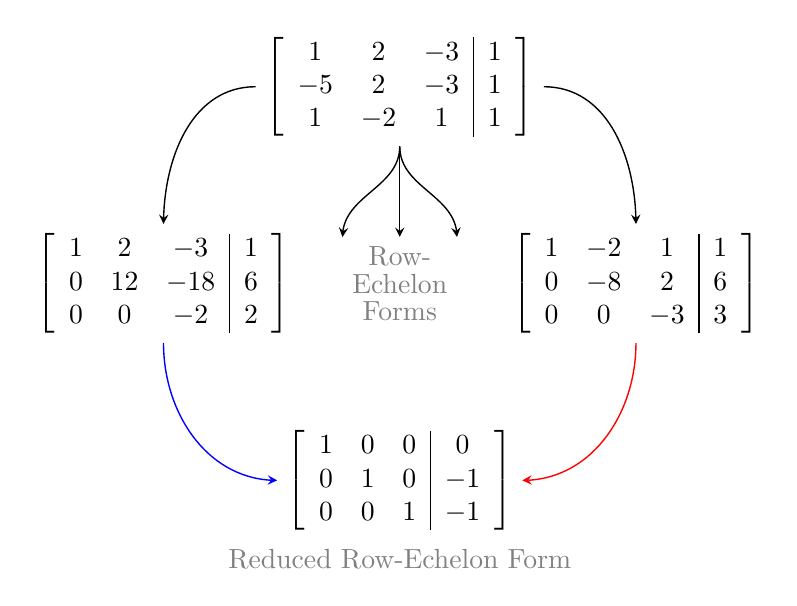
\begin{tikzpicture}
  \node[] at (0, 0)  (o)    {$\left[\begin{array}{ccc|c} 
 1&2&-3&1\\-5&2&-3&1\\1&-2&1&1
 \end{array}\right]$};
 \node[] at (-3, -2.5)  (left1)    {$\left[\begin{array}{ccc|c} 
 1&2&-3&1\\0&12&-18&6\\0&0&-2&2
 \end{array}\right]$};
 \node[] at (3, -2.5)  (right1)    {$\left[\begin{array}{ccc|c} 
 1&-2&1&1\\0&-8&2&6\\0&0&-3&3
 \end{array}\right]$};
 \node[gray] at (0, -2.5)  (c1)    {\shortstack{Row-\\Echelon\\Forms}};
 \node[] at (0, -5)  (c2)    {$\left[\begin{array}{ccc|c}  1&0&0&0\\0&1&0&-1\\0&0&1&-1
 \end{array}\right]$};
 \node[gray] at (0, -6)  (c3)    {Reduced Row-Echelon Form};
  
 \draw [->,line width=0.5pt,-stealth]  (o.west)to[out=180, in=90](left1.north);
  \draw [->,line width=0.5pt,-stealth]  (o.south)to[out=270, in=90](c1.north west);
  \draw [->,line width=0.5pt,-stealth]  (o.south)to[out=270, in=90](c1.north east);
  \draw [->,line width=0.5pt,-stealth]  (o.south)to[out=270, in=90](c1.north);
 \draw [->,line width=0.5pt,-stealth]  (o.east)to[out=0, in=90](right1.north);
 \draw [->,line width=0.5pt,-stealth,blue]  (left1.south)to[out=270, in=180](c2.west);
 \draw [->,line width=0.5pt,-stealth,red]  (right1.south)to[out=270, in=0](c2.east);
 \end{tikzpicture}
 \end{center}
We observed that a row-echelon form associated with a matrix is not unique.  In contrast, we also saw how different sequences of elementary row operations lead to the same solution set and the same reduced row-echelon form.  It turns out that the reduced row-echelon form of a matrix is unique. 


 
\begin{theorem}\label{th:uniquenessofrref} The reduced row-echelon form of a matrix is unique.
\end{theorem}
A proof of this result can be found in [Yuster].
 
The reduced row-echelon form of a matrix is an instance of a row-echelon form of the matrix.  While a given matrix may have multiple row-echelon forms, all row-echelon forms will share one characteristic: the number of nonzero rows in a row-echelon form of the given matrix will be the same.
We will prove this result in Theorem \ref{th:samenumberofnonzerorows}.
 
\section*{Gaussian and Gauss-Jordan Elimination}
 
\begin{definition}[Gaussian Elimination]\label{def:GaussianElimination}
The process of using the elementary row operations on a matrix to transform it into row-echelon form is called \dfn{Gaussian Elimination}.
\end{definition}
 
As we saw in the previous section, it is possible to follow different sequences of row operations to arrive at various row-echelon forms.  However, it was not clear whether it is {\it always possible} to find a row-echelon form.  The following algorithm takes any matrix (or augmented matrix) and transforms it into row-echelon form:
\begin{algorithm}[Gaussian Algorithm] \label{alg:gaussian}
Let $A$ be an $m\times n$ matrix.

 
Set $i=1$ initially.
\begin{itemize}
\item[] Step 1. If $A$ consists entirely of zeros, stop;  $A$ is already in row-echelon form.
 
\item[] Step 2. Otherwise, find the first column from the left containing a nonzero entry in row $i$ or below row $i$.  This column will be called a \dfn{pivot column}.  Go down the pivot column, beginning with row $i$. Pick the topmost nonzero entry and call it $a$. If $a$ is not in row $i$, switch rows so that $a$ moves to row $i$.  Now $a$ is the \dfn{leading entry} in its row.  We will also refer to $a$ as a \dfn{pivot}. 
 
\item[] Step 3. By subtracting multiples of the row containing $a$ from rows below it, make each entry below $a$ zero.
 
\item[] Step 4.  Set $i=i+1$.  If $i > m$ then stop; $A$ is in row-echelon form.
 
\end{itemize}
 
Repeat steps 1--4 on the matrix consisting of the remaining rows.
When the process stops, $A$ will be in row echelon form.
\end{algorithm}
Gaussian Algorithm guarantees that every matrix will have a row-echelon form. 


 
\begin{example}\label{ex:non-augmented}
 
Use the Gaussian Algorithm to find a row-echelon form of $A$ if $$A=\begin{bmatrix}2&4\\1&2\\-1&1\\3&5\end{bmatrix}$$
\begin{explanation}
Following Step 2, we choose the first entry, $2$, as our pivot.  We then perform step 3, using the top row to get zeros in all entries below the $2$.
$$\begin{bmatrix} \fbox{$2$}&4\\1&2\\-1&1\\3&5\end{bmatrix}
  \begin{array}{c}
  \\
  \xrightarrow{R_2-(1/2)R_1}\\
  \xrightarrow{R_3+(1/2)R_1}\\
 \xrightarrow{R_4-(3/2)R_1}\\
 \end{array}
\begin{bmatrix}2&4\\0&0\\0&3\\0&-1\end{bmatrix}
$$
The first row is now complete, and we repeat the process on the rows below it. We identify $3$ as a pivot entry in the second column and move the row containing $3$ to be directly below the first completed row.  We then use the $3$ to make each entry below the $3$ a zero. 
 
$$\begin{bmatrix}2&4\\0&0\\0&\fbox{$3$}\\0&-1\end{bmatrix}
\xrightarrow{R_2\leftrightarrow R_3}\\
\begin{bmatrix}2&4\\0&\fbox{$3$}\\0&0\\0&-1\end{bmatrix}
  \begin{array}{c}
 \\
\\
  \\
 \xrightarrow{R_4+\frac{1}{3}R_2}\\
 \end{array}
 \begin{bmatrix}2&4\\0&3\\0&0\\0&0\end{bmatrix}
$$
This time the algorithm terminates since row 3 and row 4 are zero rows.
\end{explanation}
\end{example}
  

 
 
\begin{definition}[Gauss-Jordan Elimination]\label{def:GaussJordanElimination}
The process of using the elementary row operations on a matrix to transform it into reduced row-echelon form is called \dfn{Gauss-Jordan elimination}.
\end{definition}
 
Given a matrix in row-echelon form, it is easy to bring it the reduced row-echelon form.  For example, continuing with Example \ref{ex:non-augmented}, we can start where we left off and compute $\mbox{rref}(A)$.  From our earlier computations we have:
 
$$\begin{bmatrix}2&4\\-1&1\\3&5\\1&2\end{bmatrix}\rightsquigarrow\begin{bmatrix}2&4\\0&3\\0&0\\0&0\end{bmatrix}$$
 
Now we create leading $1's$ and use them to to wipe out all non-zero entries above them.
$$\begin{bmatrix}2&4\\0&3\\0&0\\0&0\end{bmatrix}
  \begin{array}{c}
    \xrightarrow{(1/2)R_1}\\
  \xrightarrow{(1/3)R_2}\\
  \\
  \\
 \end{array}
\begin{bmatrix}1&2\\0&1\\0&0\\0&0\end{bmatrix}
  \begin{array}{c}
  \xrightarrow{R_1-2R_2}\\
\\
\\
 \\
 \end{array}
\begin{bmatrix}1&0\\0&1\\0&0\\0&0\end{bmatrix}=\mbox{rref}(A)$$
 
The following modification to the Gaussian Algorithm produces the reduced row-echelon form of a matrix.  This algorithm guarantees the existence of the reduced row-echelon form.
 
\begin{algorithm}[Gauss-Jordan Algorithm] \label{alg:gauss-jordan}
Let $A$ be an $m\times n$ matrix.
Follow the steps of the Gaussian Algorithm but modify Step 2 to create leading $1's$ by multiplying the row containing $a$ by $\frac{1}{a}$.
%Set $i=1$ initially.
%\begin{itemize}
%\item[] Step 1. If $A$ consists entirely of zeros, stop.  $A$ is already in row-echelon form.
 
%\item[] Step 2*. Otherwise, find the first column from the left containing a nonzero entry in row $i$ or below row $i$.  This column will be called a \dfn{pivot column}.  Scan the pivot column from top to bottom, starting with row $i$.  Pick the topmost nonzero entry and call it $a$.  Switch rows, if necessary, to move the row containing $a$ to row $i$.  Now $a$ is the \dfn{leading entry} in its row.  We will also refer to $a$ as a \dfn{pivot}.  Multiply the row containing $a$ by $\frac{1}{a}$ to create a leading $1$. 
 
%\item[] Step 3*. By subtracting multiples of the row containing the leading $1$ from rows {\it above} and below it, make each entry above and below the leading $1$ zero.
 
%\item[] Step 4.  Set $i=i+1$.  If $i&gt;m$ then stop, and $A$ will be in row-echelon form.
 
%\end{itemize}
 
%Repeat steps 1--4 on the matrix consisting of the remaining rows.
%When the process stops, $A$ will be in reduced row echelon form.
When the Gaussian Algorithm terminates, subtract multiples of the rows containing leading $1's$ from the rows above to make all entries above the pivots zero.
\end{algorithm}
 
 

 
\begin{example}\label{ex:gaussjordanalg}
Use the Gauss-Jordan Algorithm to solve the system
$$\begin{array}{ccccccccc}
      3x &+ &y&+&7z&= &7 \\
     5x& +&3y&+&9z&=&13\\
      2x&+ &y&+&4z&=&5
    \end{array}$$
\begin{explanation}
\begin{align*}&\left[\begin{array}{ccc|c} 
 \fbox{$3$}&1&7&7\\5&3&9&13\\2&1&4&5
 \end{array}\right]\\
 \begin{array}{c}
  \xrightarrow{\frac{1}{3}R_1}\\
\\
\\
 \end{array}
 &\left[\begin{array}{ccc|c} 
 \fbox{$1$}&1/3&7/3&7/3\\5&3&9&13\\2&1&4&5
 \end{array}\right]\\
 \begin{array}{c}
 \\
 \xrightarrow{R_2-5R_1}\\
\\
\end{array}
&\left[\begin{array}{ccc|c} 
 \fbox{$1$}&1/3&7/3&7/3\\0&4/3&-8/3&4/3\\2&1&4&5
 \end{array}\right]\\
 \begin{array}{c}
  \\
\\
 \xrightarrow{R_3-2R_1}\\
\end{array}&\left[\begin{array}{ccc|c} 
 1&1/3&7/3&7/3\\0&\fbox{$4/3$}&-8/3&4/3\\0&1/3&-2/3&1/3
 \end{array}\right]\\
 \begin{array}{c}
\\
 \xrightarrow{\frac{3}{4}R_2}\\
\\
\end{array}
&\left[\begin{array}{ccc|c} 
 1&1/3&7/3&7/3\\0&\fbox{$1$}&-2&1\\0&1/3&-2/3&1/3
 \end{array}\right]\\
 \begin{array}{c}
\\
\\
 \xrightarrow{R_3-\frac{1}{3}R_2}\\
\end{array}
&\left[\begin{array}{ccc|c} 
 1&1/3&7/3&7/3\\0&\fbox{$1$}&-2&1\\0&0&0&0
 \end{array}\right]\\
 \begin{array}{c}
 \xrightarrow{R_1-\frac{1}{3}R_2}\\
 \\
\\
\end{array}
&\left[\begin{array}{ccc|c} 
 1&0&3&2\\0&1&-2&1\\0&0&0&0
 \end{array}\right]
 \end{align*}
  
 We convert the reduced row-echelon form to a system of equations and find the solution.  The last equation contributes nothing to the system so we omit writing it down.
  
 $$\begin{array}{ccccccccc}
      x & &&+&3z&= &2 \\
     & &y&-&2z&=&1
    \end{array}$$
    The solution is
    $$x=2-3t,\quad y=1+2t,\quad z=t$$
\end{explanation}
\end{example}
The Gauss-Jordan Algorithm guarantees the existence of the reduced row-echelon form for all matrices. 
When doing computations by hand, however, the algorithm may not always be the optimal method of finding a row-echelon form or the reduced row-echelon form because the procedure often leads to fractions early in the process.
The following video shows how to arrive at the same reduced row-echelon form for the matrix in Example \ref{ex:gaussjordanalg} without doing any fraction arithmetic.  You will see that we still employ row operations, but in a different order.
 
\youtube{76Y41ncuLeQ}
 
The video highlights the fact that regardless of what sequence of elementary row operations we take to arrive at the reduced row-echelon form, the end result is the same. 


 
\subsection*{Rank}
 
As stated in Theorem \ref{th:uniquenessofrref}, the reduced row-echelon form of a matrix $A$ is uniquely determined by $A$. That is, no matter which series of row operations is used to transform $A$ to its reduced row-echelon matrix, the result will always be the same matrix. In contrast, this is not true for row-echelon matrices: different sequences of row operations can transform the same matrix $A$ to different row-echelon matrices. However, it is true that the number $r$ of nonzero rows must be the same in each of these row-echelon matrices, as we will see in Theorem \ref{th:dimofrowA}. Hence, the number $r$ depends only on $A$ and not on the way in which $A$ is carried to row-echelon form. 
 
\begin{example}\label{ex:rowechofA}
Matrices (\ref{eq:ref1}) and (\ref{eq:ref2}) of Exploration \ref{init:gaussianelim1} are both row-echelon forms of $A$.  Both matrices have three nonzero rows.  The same is true for $\mbox{rref}(A)$. 
\end{example}
 
\begin{definition}\label{def:rankofamatrix}
The \dfn{rank} of matrix $A$, denoted by $\mbox{rank}(A)$, is the number of nonzero rows that remain after we reduce $A$ to row-echelon form by elementary row operations.
\end{definition}
 
\begin{example}\label{ex:rankofA1}
Compute the rank of
$$A = 
\begin{bmatrix}
    1 & 1 & -1 & 4 \\
    2 & 1 &  3 & 0 \\
    0 & 1 & -5 & 8
\end{bmatrix}$$
 
\begin{explanation}
A reduction of $A$ to row-echelon form is
$$
A = 
\begin{bmatrix}
1 & 1 & -1 & 4 \\
2 & 1 &  3 & 0 \\
0 & 1 & -5 & 8
\end{bmatrix} \rightsquigarrow\begin{bmatrix}
1 & 1 & -1 & 4 \\
0 & -1 &  5 & -8 \\
0 &  0 & 0 & 0
\end{bmatrix}
$$
Because the row-echelon form has two nonzero rows, $\mbox{rank}(A) = 2$.
\end{explanation}
\end{example}
 
\begin{theorem}\label{th:rankandsolutions}
Suppose a system of $m$ equations in $n$ variables is consistent, and that the rank of the {\it coefficient} matrix is $r$.
 
\begin{enumerate}
\item The set of solutions involves exactly $n - r$ parameters, corresponding to $n-r$ free variables.
 
\item If $r < n$, the system has infinitely many solutions.
 
\item If $r = n$, the system has a unique solution.
 
\end{enumerate}
\end{theorem}


 
\begin{proof}
The fact that the rank of the coefficient matrix is $r$ means that there are exactly $r$ leading variables in the coefficient matrix, and hence exactly $n - r$ nonleading variables. The nonleading variables are called free variables.  All free variables are assigned parameters, so the set of solutions involves exactly $n - r$ parameters. Hence if $r < n$, there is at least one parameter, and so infinitely many solutions. If $r = n$, there are no parameters and the resulting solution is unique.
\end{proof}
 
Theorem \ref{th:rankandsolutions} shows that, for any system of linear equations, exactly three possibilities exist:
 
\begin{enumerate}
 
\item Unique solution. This occurs when every variable is a leading variable.
 
\item Infinitely many solutions. This occurs when the system is consistent and there is at least one nonleading variable, so at least one parameter is involved.
 
\item No solution.  This occurs when a row $\left[\begin{array}{cccc|c}  0&0&\ldots &0&1
 \end{array}\right]$ appears in the row-echelon form. Such a row corresponds to an equation with no solutions. (See Example \ref{ex:nosolutionssys}.)
 
\end{enumerate}
 

 
 
\section*{Practice Problems}
 
\begin{problem}\label{prob:same_rref}
Show that applying Gauss-Jordan elimination to the matrix in Exploration \ref{init:gaussianelim2} yields the same reduced row-echelon form as the matrix we obtained in Exploration \ref{init:gaussianelim1}.
\end{problem}
 
\begin{problem}\label{prob:twowaystorref1}
Follow the indicated steps of the Gauss-Jordan algorithm to transform the matrix to its reduced row-echelon form.  Steps will unfold automatically as you enter correct answers.
 
$$\left[\begin{array}{ccc|c}  2&1&1&3\\-1&0&1&2\\1&1&-2&0
  \end{array}\right]$$
 
 \begin{prompt}  $\frac{1}{2}R_1\rightarrow R_1$.
$$ \left[\begin{array}{ccc|c}   \answer{1}&\answer{1/2}&\answer{1/2}&\answer{3/2}\\-1&0&1&2\\1&1&-2&0
  \end{array}\right]$$
 \end{prompt}
 
 \begin{problem}
 \begin{prompt} $R_1+R_2\rightarrow R_2$.
$$ \left[\begin{array}{ccc|c}  1&1/2&1/2&3/2\\\answer{0}&\answer{1/2}&\answer{3/2}&\answer{7/2}\\1&1&-2&0
  \end{array}\right]$$
 \end{prompt}
 \begin{problem}
 \begin{prompt} $R_3-R_1\rightarrow R_3$.
$$ \left[\begin{array}{ccc|c}   1&1/2&1/2&3/2\\0&1/2&3/2&7/2\\\answer{0}&\answer{1/2}&\answer{-5/2}&\answer{-3/2}
  \end{array}\right]$$
 \end{prompt}
  \begin{problem}
  \begin{prompt} $2R_2\rightarrow R_2$.
$$ \left[\begin{array}{ccc|c}   1&1/2&1/2&3/2\\\answer{0}&\answer{1}&\answer{3}&\answer{7}\\0&1/2&-5/2&-3/2
 \end{array}\right]$$
\end{prompt}
 \begin{problem}
 \begin{prompt} $R_3-\frac{1}{2}R_2\rightarrow R_3$.
$$ \left[\begin{array}{ccc|c} 
1&1/2&1/2&3/2\\0&1&3&7\\\answer{0}&\answer{0}&\answer{-4}&\answer{-5}
  \end{array}\right]$$
 \end{prompt}
 \begin{problem}
 \begin{prompt} $-\frac{1}{4}R_3\rightarrow R_3$.
$$\left[\begin{array}{ccc|c}    1&1/2&1/2&3/2\\0&1&3&7\\\answer{0}&\answer{0}&\answer{1}&\answer{5/4}
  \end{array}\right]$$
 \end{prompt}
 \begin{problem}
 \begin{prompt} $R_2-3R_3\rightarrow R_2$.
$$ \left[\begin{array}{ccc|c} 
1&1/2&1/2&3/2\\\answer{0}&\answer{1}&\answer{0}&\answer{13/4}\\0&0&1&5/4
  \end{array}\right]$$
 \end{prompt}
 \begin{problem}
 \begin{prompt} $R_1-\frac{1}{2}R_3\rightarrow R_1$.
$$ \left[\begin{array}{ccc|c} 
\answer{1}&\answer{1/2}&\answer{0}&\answer{7/8}\\0&1&0&13/4\\0&0&1&5/4
 \end{array}\right]$$
  \end{prompt}
  \begin{problem}
 \begin{prompt} $R_1-\frac{1}{2}R_2\rightarrow R_1$.
$$ \left[\begin{array}{ccc|c} 
 \answer{1}&\answer{0}&\answer{0}&\answer{-3/4}\\0&1&0&13/4\\0&0&1&5/4
  \end{array}\right]$$
  \end{prompt}
 \end{problem}
  \end{problem}
  \end{problem}
  \end{problem}
  \end{problem}
  \end{problem}
  \end{problem}
 \end{problem}
 \end{problem}
  
 
 
 
\begin{problem}
Find the rank of each matrix.
\begin{problem}\label{prob:rankofmat1}
$$A=\begin{bmatrix}4&3&-1\\-8&-6&2\end{bmatrix}$$
Answer:
 
$$\mbox{rank}(A)=\answer{1}$$
\end{problem}
 
\begin{problem}\label{prob:rankofmat2}
$$B=\begin{bmatrix}1&1\\2&-2\\3&-1\end{bmatrix}$$
Answer:
 
$$\mbox{rank}(B)=\answer{2}$$
\end{problem}
 
\begin{problem}\label{prob:rankofmat3}
$$C=\begin{bmatrix}1&0&1\\2&1&3\\0&1&-2\end{bmatrix}$$
Answer:
 
$$\mbox{rank}(C)=\answer{3}$$
\end{problem}
 
\begin{problem}\label{prob:rankofmat4}
$$D=\begin{bmatrix}1&1&2\\-1&-2&1\\1&0&5\end{bmatrix}$$
Answer:
 
$$\mbox{rank}(D)=\answer{2}$$
\end{problem}
\end{problem}
 
\begin{problem}\label{prob:rankofmat5}
Suppose $A$ is a $5\times 7$ matrix.  Which of the following can be true?
\begin{multipleChoice}
 \choice{$\mbox{rank}(A)=7$}
 \choice{$\mbox{rank}(A)=6$}
 \choice[correct]{$\mbox{rank}(A)=5$}
 \choice{All of the above}
 \end{multipleChoice}
\end{problem}
 
\begin{problem}\label{prob:4eq5un}
Suppose a linear system has $4$ equations and $5$ unknowns.  Which of the following is NOT a possibility?
\begin{multipleChoice}
  \choice[correct]{The system has a unique solution}
 \choice{The system has no solutions}
 \choice{The system has infinitely many solutions}
 \end{multipleChoice}
\end{problem}
 
\begin{problem}\label{prob:leadones}
Suppose $A$ is a matrix such that $\mbox{rref}(A)$ has $5$ leading $1's$.  What do we know to be true about $A$?  Select ALL that apply.
\begin{selectAll}
 \choice[correct]{$\mbox{rank}(A)=5$}
 \choice[correct]{$A$ has at least $25$ entries}
 \choice[correct]{Any row-echelon form of $A$ will have exactly $5$ nonzero rows}
 \choice{Some row-echelon forms of $A$ may have more than $5$ nonzero rows}
 \choice{Some row-echelon forms of $A$ may have less than $5$ nonzero rows}
 \end{selectAll}
\end{problem}
 
\begin{problem}\label{prob:rankaugvscoeff}
In this problem we will discuss how the rank of the {\it coefficient matrix} associated with a linear system compares to the rank of the {\it augmented matrix} associated with the system. 
\begin{enumerate}
\item Explain why the rank of the augmented matrix has to be greater than or equal to the rank of the coefficient matrix.
    \item Prove that for a {\it consistent} system the rank of the coefficient matrix will be the same as the rank of the {\it augmented} matrix.
    \item Give an example of an inconsistent system for which the rank of the augmented matrix is greater than the rank of the coefficient matrix.
    \item Can the rank of an augmented matrix be greater than the number of variables?
    \item Is the following statement true?
     
    ``If the rank of the augmented matrix associated with a linear system is greater than the rank of the coefficient matrix, then the system is inconsistent."
\end{enumerate}
\end{problem}
 
\section*{Text Source}
The section on Rank is an adaptation of Section 1.2 of Keith Nicholson's \href{https://open.umn.edu/opentextbooks/textbooks/linear-algebra-with-applications}{\it Linear Algebra with Applications}.
 
W. Keith Nicholson, {\it Linear Algebra with Applications}, Lyryx 2018, Open Edition, p 15-17.
 
\section*{Bibliography}
 
[Yuster] Thomas Yuster, The Reduced Row Echelon Form of a Matrix is Unique: a
Simple Proof, Mathematics Magazine, vol. 57, no. 2 (Mar. 1984), pp. 93-94.
 
  
\end{document}